%%%%%%%%%%%%%%%%%%%%%%%%%%%%%%%%%%%%%%%%%%%%%%%%%%%%%%%%%%%%%%%%%%%%%%%%%%
\begin{figure*}[tbp!]
%\vspace{-2mm}
\centering
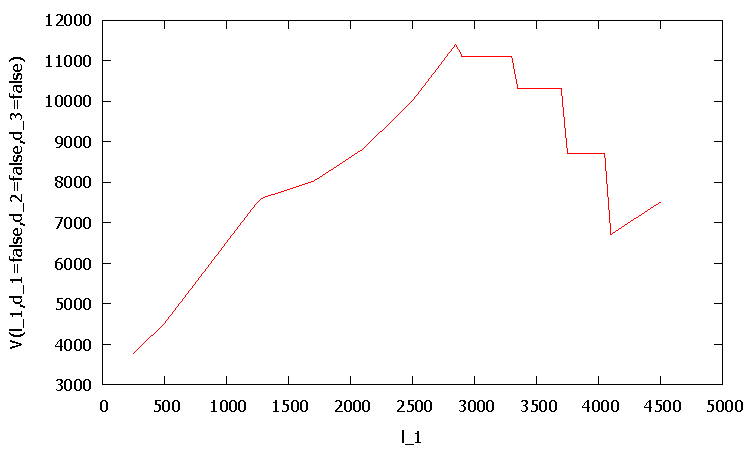
\includegraphics[width=0.33\textwidth]{Figures/reserV7.pdf}
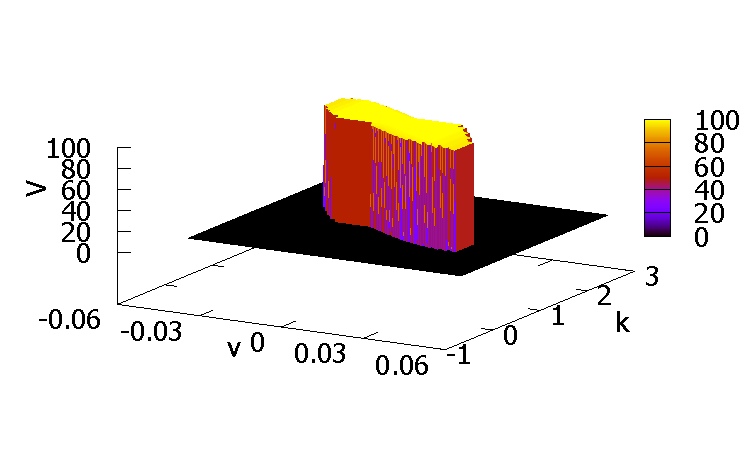
\includegraphics[width=0.33\textwidth]{Figures/telesV4.pdf}
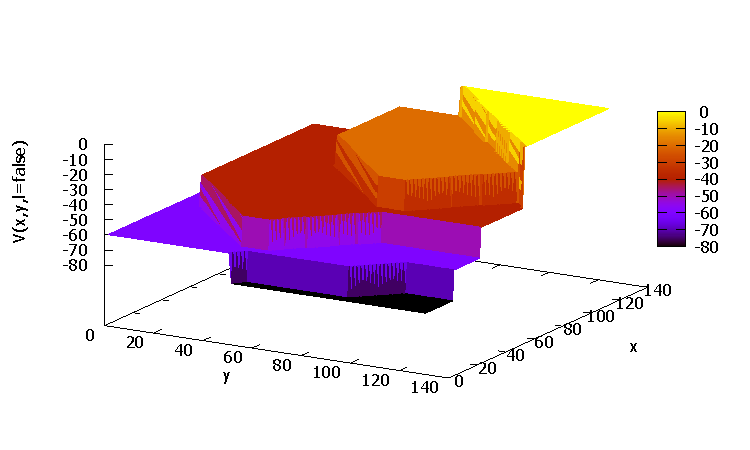
\includegraphics[width=0.33\textwidth]{Figures/uavV4.pdf}
\vspace{-2mm}
\caption{\footnotesize
{\it (left)}  $V^7(l_1,d_1=false,d_2=false,d_3=false)$ \textsc{Reservoir Control} problem;
{\it (middle)} $V^4(k,v,z=true,g=false)$ \textsc{Space Telescope Control} problem.
{\it (right)}  $V^4(x,y,l=false)$\textsc{UAV Navigation} problem;
}
\label{fig:Value}
%\vspace{-5mm}
\end{figure*}
%%%%%%%%%%%%%%%%%%%%%%%%%%%%%%%%%%%%%%%%%%%%%%%%%%%%%%%%%%%%%%%%%%%%%%%%%%


%%%%%%%%%%%%%%%%%%%%%%%%%%%%%%%%%%%%%%%%%%%%%%%%%%%%%%%%%%%%%%%%%%%%%%%%%%
\begin{figure}[tbp!]
\vspace{-2mm}
\centering

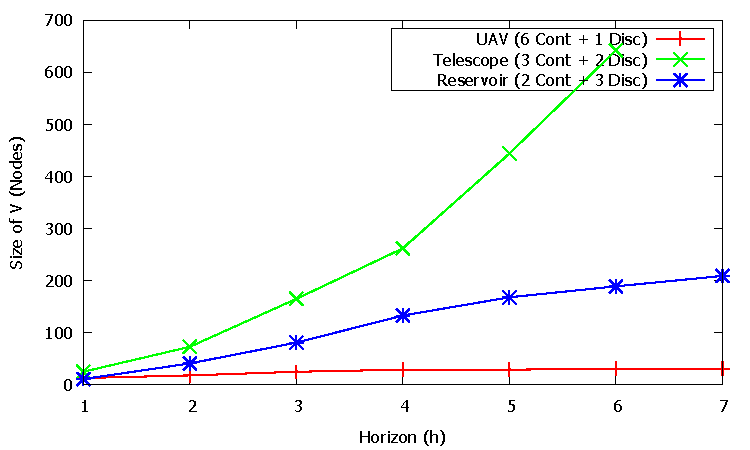
\includegraphics[width=0.42\textwidth]{Figures/Nodes.pdf}\\
\vspace{-2mm}
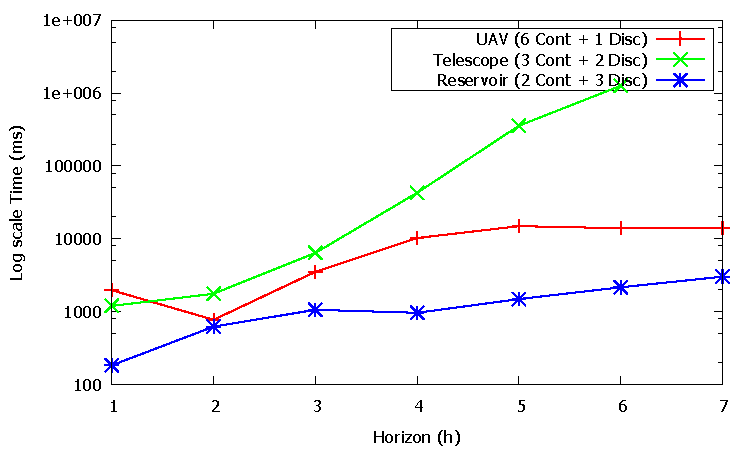
\includegraphics[width=0.42\textwidth]{Figures/Time.pdf}

\vspace{-2mm}
\caption{\footnotesize Space and elapsed time (between current and previous horizon) vs. horizon.
}
\label{fig:SpaceTime}
\vspace{-4mm}
\end{figure}
%%%%%%%%%%%%%%%%%%%%%%%%%%%%%%%%%%%%%%%%%%%%%%%%%%%%%%%%%%%%%%%%%%%%%%%%%%

\label{sec:results}

We evaluated RH-MDP on the \textsc{Reservoir Control} problem used as a running example,
\textsc{UAV Navigation} problem  and
\textsc{Space Telescope Control} problem --- described below.\footnote{While
space limitations prevent a self-contained
description of all domains, we note that all Java source code and a
human/machine readable file format for all domains needed to reproduce
the results in this paper can be found online at
\texttt{http://code.google.com/p/xadd-inference}.}

Figure \ref{fig:Value} (left) shows the value function for the \textsc{Reservoir Control} problem in horizon seven. We can observe that we can gain  11000 units if the reservoir begins with a water level approximately equal to 3000 when the four first day are dry and the following three are rainy.

%{\bf \textsc{Reservoir Control}:} Reservoir management is a well-studied in
%OR~\cite{Mahootchi2009,Yeh1985}.  In this domain we decided between
%\emph{drain} (or \emph{not drain}) each reservoir to maximize
%electricity revenue over the decision-stage horizon while avoiding
%reservoir overflow and underflow.

%We solve a 2-reservoir problem with
%levels $(l_1,l_2)\in [0,\infty]^2$ with reward penalties for
%overflow and underflow and a reward gain of 1, i.e.:


%{\footnotesize
%\begin{align*}
%R & = \begin{cases}
%(l_1 \leq 4500) \wedge (l_2 \leq 4500) \wedge (l_1 \geq 200) \wedge (l_2 \geq 200) &:1\\
%else &: -\infty\\
%\end{cases}
%\end{align*}}


%The electricity is generated in periods when the $\mathit{drain}()$ action
%drains water from $l_2$ to $l_1$, the other action is
%$\mathit{no}$-$\mathit{drain}()$); we assume a daily control,  four days are wet and the next four days are dry (we use three discrete variables to %count the day $d_1$, $d_2$, $d_3$), the rainfall
%replenishment depends on that and is modeled by the noise:
%{\footnotesize
%\begin{align*}
%n & = \begin{cases}
%(d_1) \wedge (n \leq 2000) \wedge (n \geq 1200) &:legal\\
%\neg (d_1) \wedge (n \leq 400) \wedge (n \geq 0) &:legal\\
%else &: illegal\\
%\end{cases}
%\end{align*}}


%The transition function for levels of the $\mathit{drain}$ action are
%{\footnotesize
%\begin{align*}
%l_1' & =(n + l_1 - 2800 + 2000) \\
%l_2'& =(n + l_2 - 2000)
%\end{align*}}
%while for $\mathit{no}$-$\mathit{drain}$ action, the $\mathit{2000}$ term is dropped.

{\bf \textsc{Space Telescope Control}:} We have extended the problem of slewing a space telescope
in order to look a new objective given in \cite{DLohr:2012}. This problem has six actions $a_0, \cdots ,a_5$ that change the angle $k$ and the angular rate $v$. The transition function for $a_5$ action, when $v < 1$ $\frac{deg}{seg}$ and the $z= false$ is:

{\footnotesize
\begin{align*}
k' & =( k + 40.55*v) \\
v'& =(2/3 v + n) \\
z'& =( true ),
\end{align*}}

Note that we assume a noise in the transition function of the angular rate for $a_5$, since this action is the only one that changes the zoom of the telescope during the slew. The noise is given by:

{\footnotesize
\begin{align*}
n & = \begin{cases}
\neg (z) \wedge (n \leq 0.04*v) \wedge (n \geq -0.04*v) &:-\infty\\
else &: +\infty\\
\end{cases}
\end{align*}}

The reward for actions $a_0, \cdots ,a_5$ is given by

{\tiny
\begin{align*}
R & = \begin{cases}
(z) \wedge (v \leq 0.02) \wedge (k \leq 1.683) \wedge (v \geq -0.02) \wedge (k \geq 1.283) &:100\\
else &: -cost\\
\end{cases}
\end{align*}}

where cost of action $a_0$  is 0, $1$ for actions $a_i$ $i \in \{1,2,3,4\}$ and $10$ for action $a_5$.
Figure \ref{fig:Value} (right) shows the value function for the horizon four. We can see that there are relative few states that have a policy to achieve a goal (a reward of 0) with high certainty over this horizon.


Figure \ref{fig:Value} (middle) shows the value function for the horizon four. We can observe  that there are states with low angular rate ($-0.04\leq v \leq 0.04$ approximately) that have a policy to achieve a goal (a reward of 100) with high certainty over this horizon.


{\bf \textsc{UAV Navigation}:}
In this problem a UAV needs to be able to plan
trajectories that take the aircraft from its current location to
a goal given constraints on time or fuel
consumption and known areas of turbulence.

The state consist of UAV´s continuous position $x$ and $y$.
In a given time step, the UAV may move a continuous distance $ax \in [-40,40]$ and $ay \in [-40,40]$. The turbulence introduces a noise $nx$ and $ny$ respectively in the movement, given by:

{\footnotesize
\begin{align*}
nx & = \begin{cases}
(y \geq 50 + x) \wedge (nx \leq -20) \wedge (nx \geq 20) &:-\infty\\
(y < 50 + x) \wedge (nx \leq -5) \wedge (nx \geq 5) &:-\infty\\
else &: +\infty\\
\end{cases}
\end{align*}}

{\footnotesize
\begin{align*}
ny & = \begin{cases}
(y \geq 50 + x) \wedge (ny \leq -20) \wedge (ny \geq 20) &:-\infty\\
(y < 50 + x) \wedge (ny \leq -5) \wedge (ny \geq 5) &:-\infty\\
else &: +\infty\\
\end{cases}
\end{align*}}
The UAV goal is to achieve the region $x+y > 200$. It receives a reward penalty ($-\infty$) for being in positions  from which a UAV with a given amount of fuel reserves cannot return to its landing strip. If the UAV is not in the goal position ($\neg l$), the action cost is 20:

%added
{\footnotesize
\begin{align*}
R & = \begin{cases}
(l) \wedge (x \leq 130) \wedge (y \leq 130) \wedge (x \geq 0) \wedge (y \geq 0) &:0\\
(\neg l) \wedge (x \leq 130) \wedge (y \leq 130) \wedge (x \geq 0) \wedge (y \geq 0) &:-20\\
else &: -\infty\\
\end{cases}
\end{align*}}

Figure \ref{fig:Value} (right) shows the value function for the horizon four. We can see that there are relative few states that have a policy to achieve a goal (a reward of 0) with high certainty over this horizon.


Figure \ref{fig:SpaceTime} shows the time and space for each of the solved problems. The \textsc{UAV Navigation} problem has more continuous variables, however we can see that it is easier to solve than the \textsc{Space Telescope Control}, one possible reason is that this last problem has more actions and requires more operations with float numbers.
